\documentclass[tikz,border=3pt]{standalone}
\usepackage[utf8]{inputenc}
\usepackage[T1]{fontenc}
\usepackage{lmodern}
\renewcommand{\familydefault}{\sfdefault}
\usepackage{sansmath}\sansmath
\usepackage{chemfig}
\usepackage{pgfplots}\pgfplotsset{compat=1.18,/pgf/number format/use comma,/pgf/number format/1000 sep={.}}
\usetikzlibrary{arrows.meta,calc,positioning,decorations.pathmorphing,patterns}
% paleta del sitio
\definecolor{nar}{HTML}{E8680C}\definecolor{narc}{HTML}{FFB35C}\definecolor{hielo}{HTML}{FFF3E8}
\definecolor{tinta}{HTML}{1D1D1F}\definecolor{gris}{HTML}{6E6E73}\definecolor{lila}{HTML}{7C5CF0}
\definecolor{azul}{HTML}{2F6FD6}\definecolor{menta}{HTML}{17A673}\definecolor{coral}{HTML}{E8342A}
\begin{document}
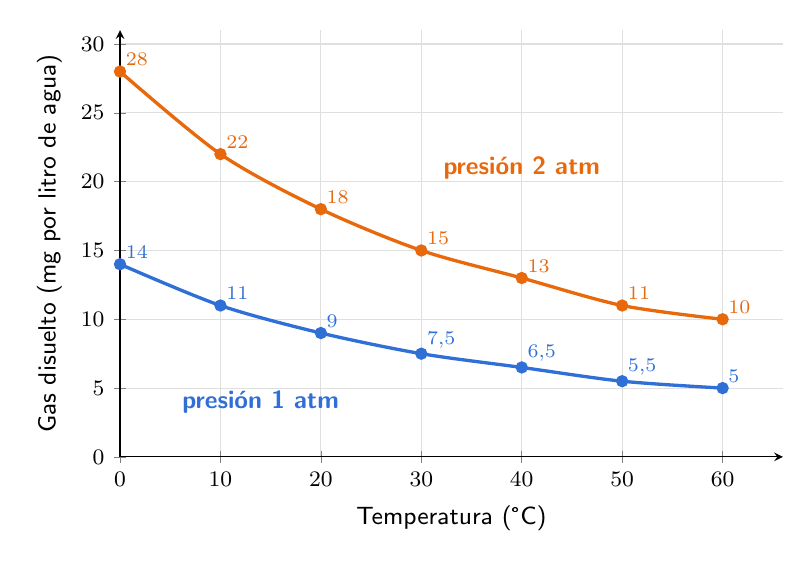
\begin{tikzpicture}[font=\small]
\begin{axis}[width=10cm,height=7cm,xmin=0,xmax=66,ymin=0,ymax=31,
  xtick={0,10,...,60},ytick={0,5,...,30},
  grid=major,major grid style={gray!25},axis lines=left,
  xlabel={Temperatura (°C)},ylabel={Gas disuelto (mg por litro de agua)},
  ylabel style={font=\small},xlabel style={font=\small},tick label style={font=\footnotesize},
  nodes near coords,every node near coord/.append style={font=\scriptsize,anchor=south west,inner sep=1.5pt}]
\addplot[nar,very thick,smooth,mark=*,mark size=1.6pt] coordinates {(0,28)(10,22)(20,18)(30,15)(40,13)(50,11)(60,10)};
\addplot[azul,very thick,smooth,mark=*,mark size=1.6pt] coordinates {(0,14)(10,11)(20,9)(30,7.5)(40,6.5)(50,5.5)(60,5)};
\node[nar,font=\small\bfseries] at (axis cs:40,21) {presión 2 atm};
\node[azul,font=\small\bfseries] at (axis cs:14,4) {presión 1 atm};
\end{axis}
\end{tikzpicture}
\end{document}
